\section{Background: Domain-specific languages in a nutshell}
\label{sec:background}

\subsubsection{Specification:} Like general purpose languages (GPLs), DSLs are defined in terms of syntax and semantics \cite{Harel:2004b}. Hence, the specification of a DSL is a tuple $<syn,sem,M_{syn\leftarrow sem}>$ \cite{Combemale:2013}. The parameter $syn$ (the \textit{\textbf{syn}tax}) refers to the structure of the DSL and specifies each language construct in terms of its name and the relationships it has with other language constructs. In turn, the parameter $sem$ (the \textit{\textbf{sem}antics}) refers to the meaning of the language constructs. This meaning corresponds to the dynamic behavior that establishes the manner in which language constructs are manipulated at runtime. Finally, the parameter $M_{syn\leftarrow sem}$ refers to the mapping between the language constructs and the semantics. 
 

\vspace{-3mm}
\subsubsection{Technological space:} Currently, there are diverse techniques available for the implementation of syntax and semantics of DSLs \cite{Mernik:2005b}. Language designers can, for example, choose between using context-free grammars or metamodels as specification formalism for syntax. Similarly, there are at least three methods for expressing semantics: operationally, denotationally, and axiomatically \cite{Mosses:2001}. In this paper we are interested on DSLs which syntax is specified by means of metamodels and semantics is specified operationally as a set methods (a.k.a, \textit{domain-specific actions} \cite{Combemale:2013}). Each language construct is specified by means a metaclass and the relationship between language constructs are specified as references between metaclasses. In turn, domain-specific actions are specified as java-like methods that are allocated in each metaclass.
 
\vspace{-3mm}
\subsubsection{Implementation:} In order to implement a DSL, language designers need a tool set that offer capabilities to specify a DSL according to the selected technological space. This kind of tool sets are provided by language workbenches (such as Eclipse Modeling Framework or MetaEdit+) that provide meta-languages for where syntax and semantics can be expressed. The ideas presented in this paper are implemented in an Eclipse-based language workbench. In particular, metamodels are specified in the Ecore language whereas domain-specific actions are specified as methods in Xtend programming language\footnote{\url{http://www.eclipse.org/xtend/}}. The mapping between metaclasses and domain-specific actions is specified by using the notion of aspect introduced by the Kermeta 3\footnote{\url{https://github.com/diverse-project/k3/wiki/Defining-aspects-in-Kermeta-3}} and Melange\footnote{\url{http://melange-lang.org/}} as explained in \cite{degueule:2015}. 

\vspace{-3mm}
\subsubsection{A simple DSL:} Let us illustrate this idea by using a simple example. Consider the metamodel introduced at the top of Figure \ref{fig:k3-example}. It is a metamodel for a simple language for finite state machines. It contains thee classes \texttt{StateMachine}, \texttt{State}, and \texttt{Transition}; The class \texttt{StateMachine} contains both states and transitions which is represented with containment references. In turn, the code snippets at the bottom of Figure \ref{fig:k3-example} introduce some operational semantics to this metamodel by using K3. Note that the main feature of K3 is the notion of aspect that permits to weave the operational semantics defined in a Xtend class to a metamodel defined in Ecore. In our example, the metaclass \texttt{StateMachine} is enriched with the operation \texttt{eval()} that contains a loop that sequentially invokes the operation defined for the class \texttt{State}. This operation is also defined by using one aspect. The metaclass \texttt{Transition} is enriched with the operation \texttt{fire()}.

\begin{figure}
\centering
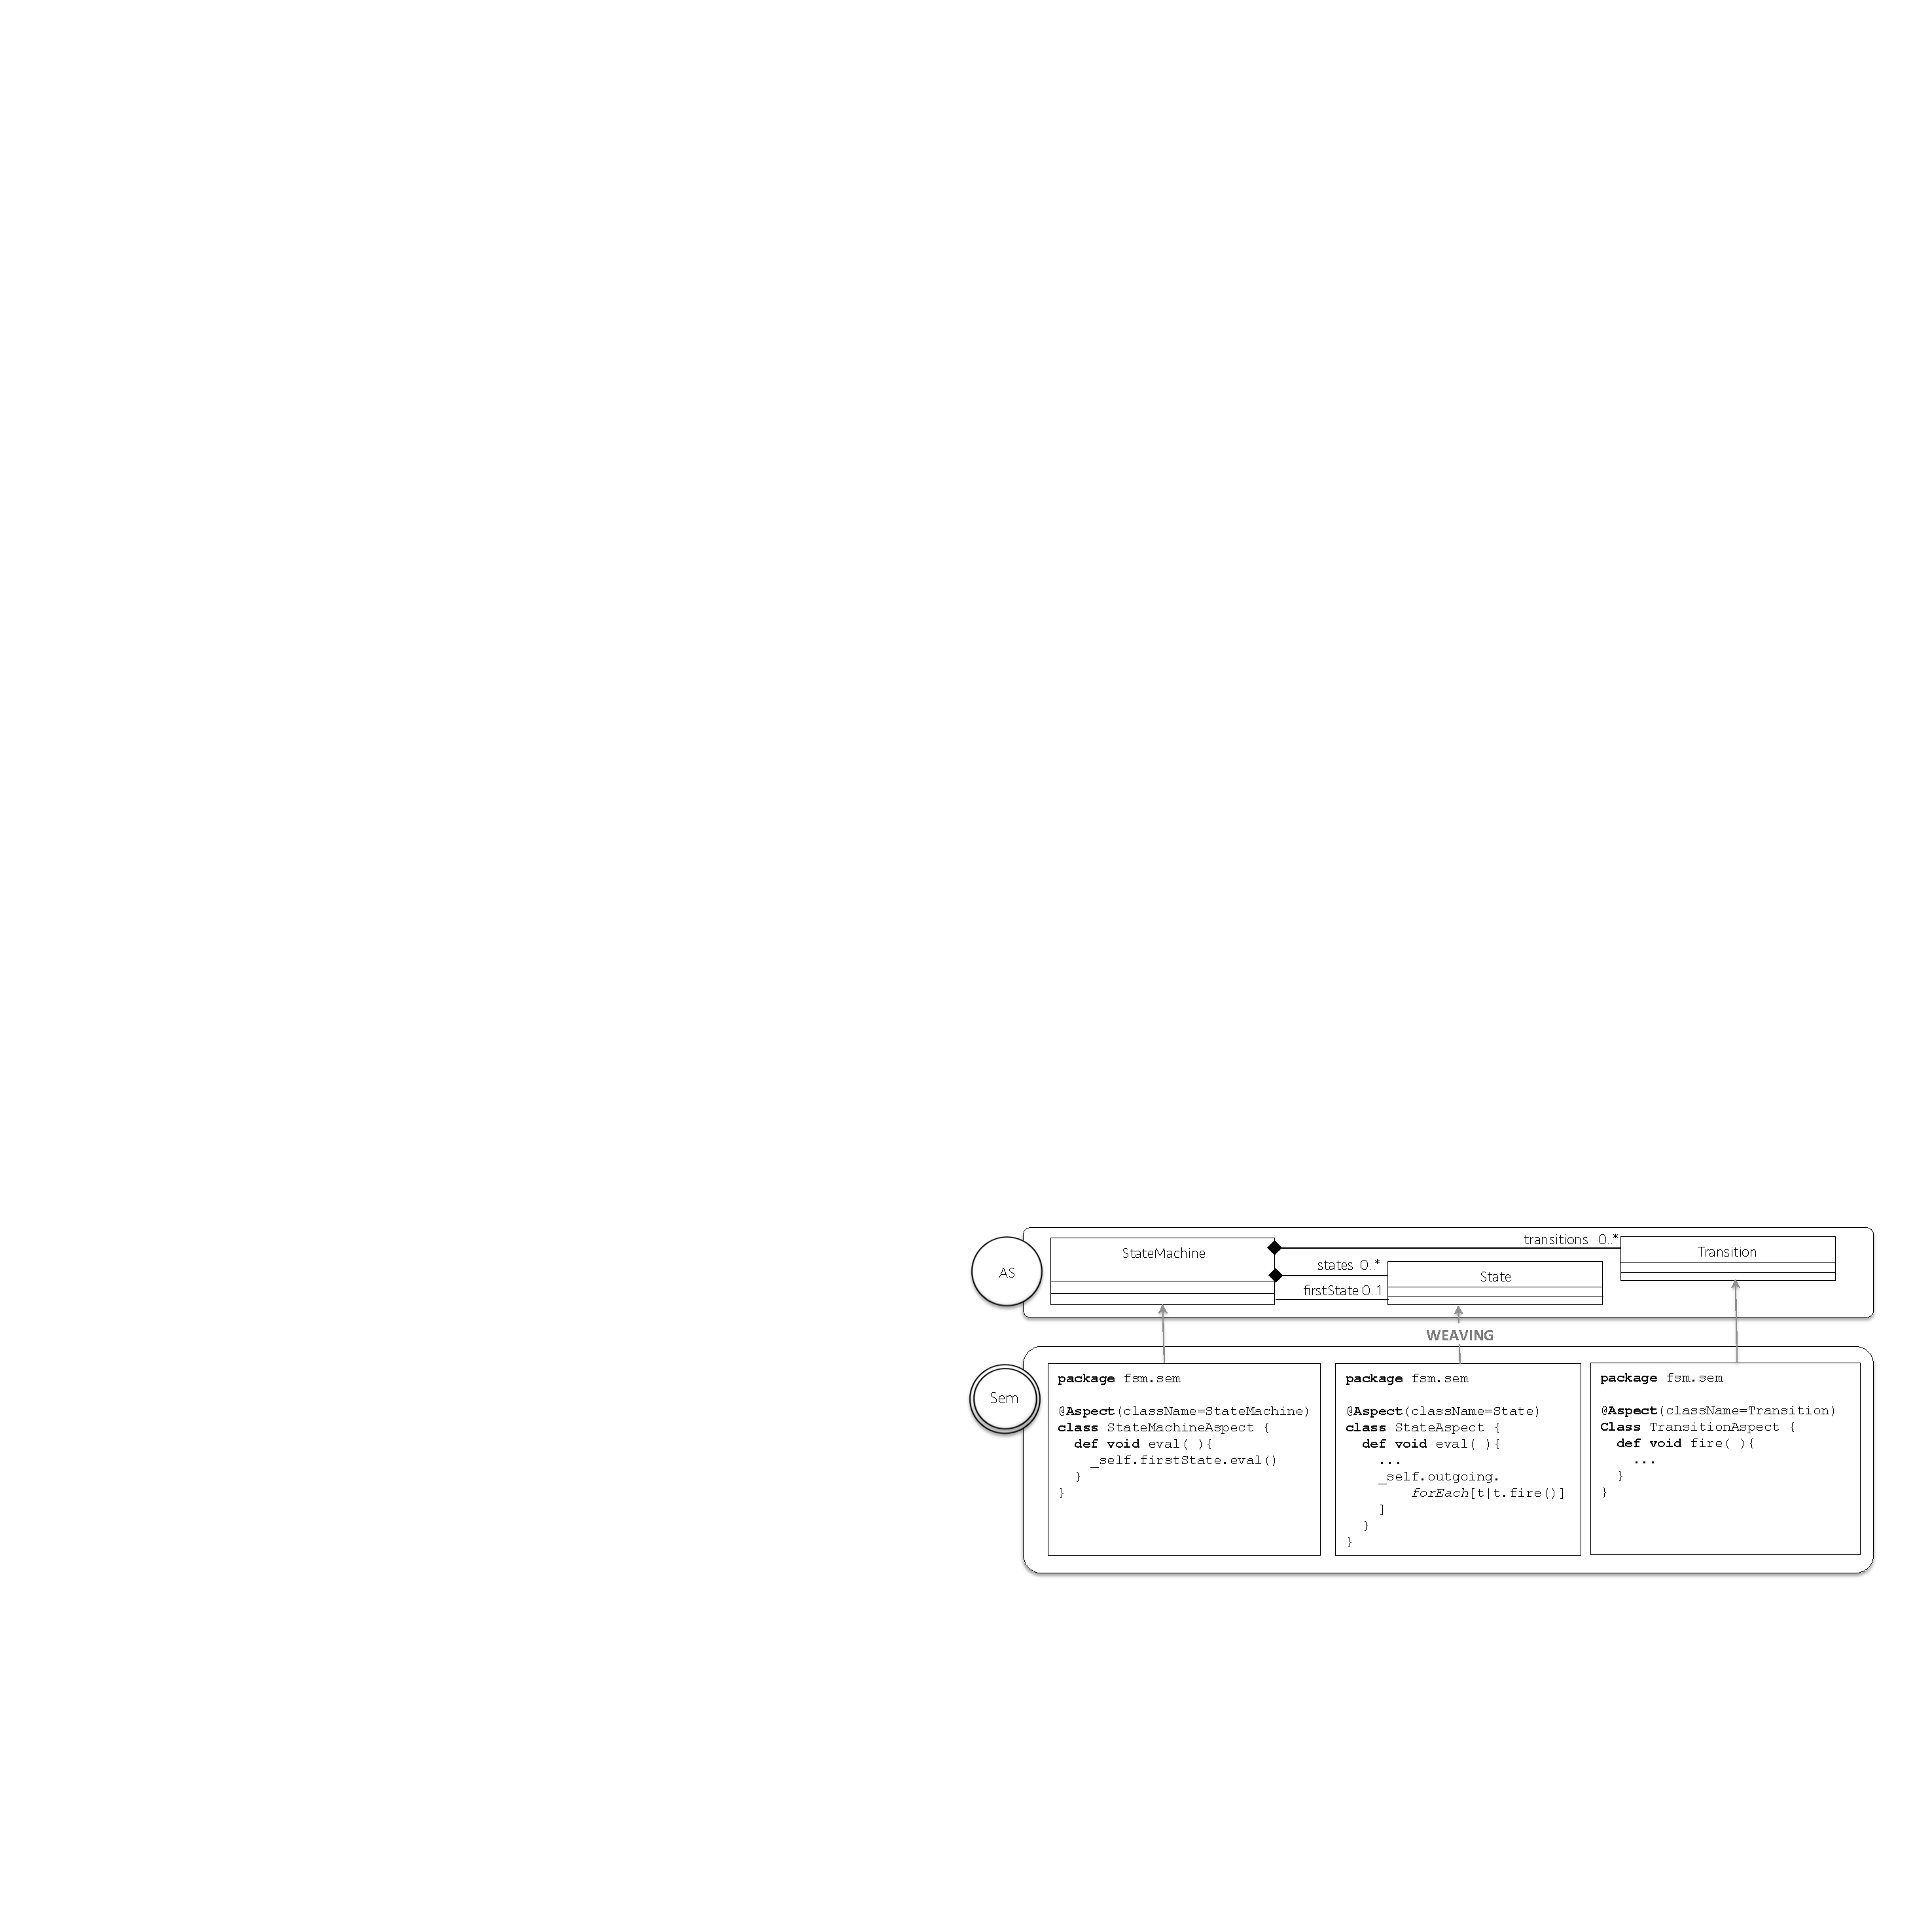
\includegraphics[width=1\linewidth]{images/k3-example-fig}
\caption{A simple FSM language}
\label{fig:k3-example}
\end{figure}

%As said above, we use Melange to integrate and execute the definitions of the abstract syntax and semantics of a DSL. Melange is a language for modeling in the large that facilitates the integration of the different artifacts that compose the specification of a DSL. Listing \ref{lst:fsm} illustrates the use of Melange. At the left we have an abstract representation of a language that is composed of a metamodel and three aspects implementing the semantics. At the right of the figure we have the corresponding Melange script.
 
%\vspace{4mm}
%\begin{lstlisting}[caption=Melange script for a simple FSM language, label=lst:fsm]
%language FSM {
%    syntax "fsm.mm/models/fsm.ecore"
%    
%    with fsm.sem.StateMachineAspect
%    with fsm.sem.StateAspect
%    with fsm.sem.TransitionAspect
%}
%\end{lstlisting}

%\begin{figure}
%\centering
%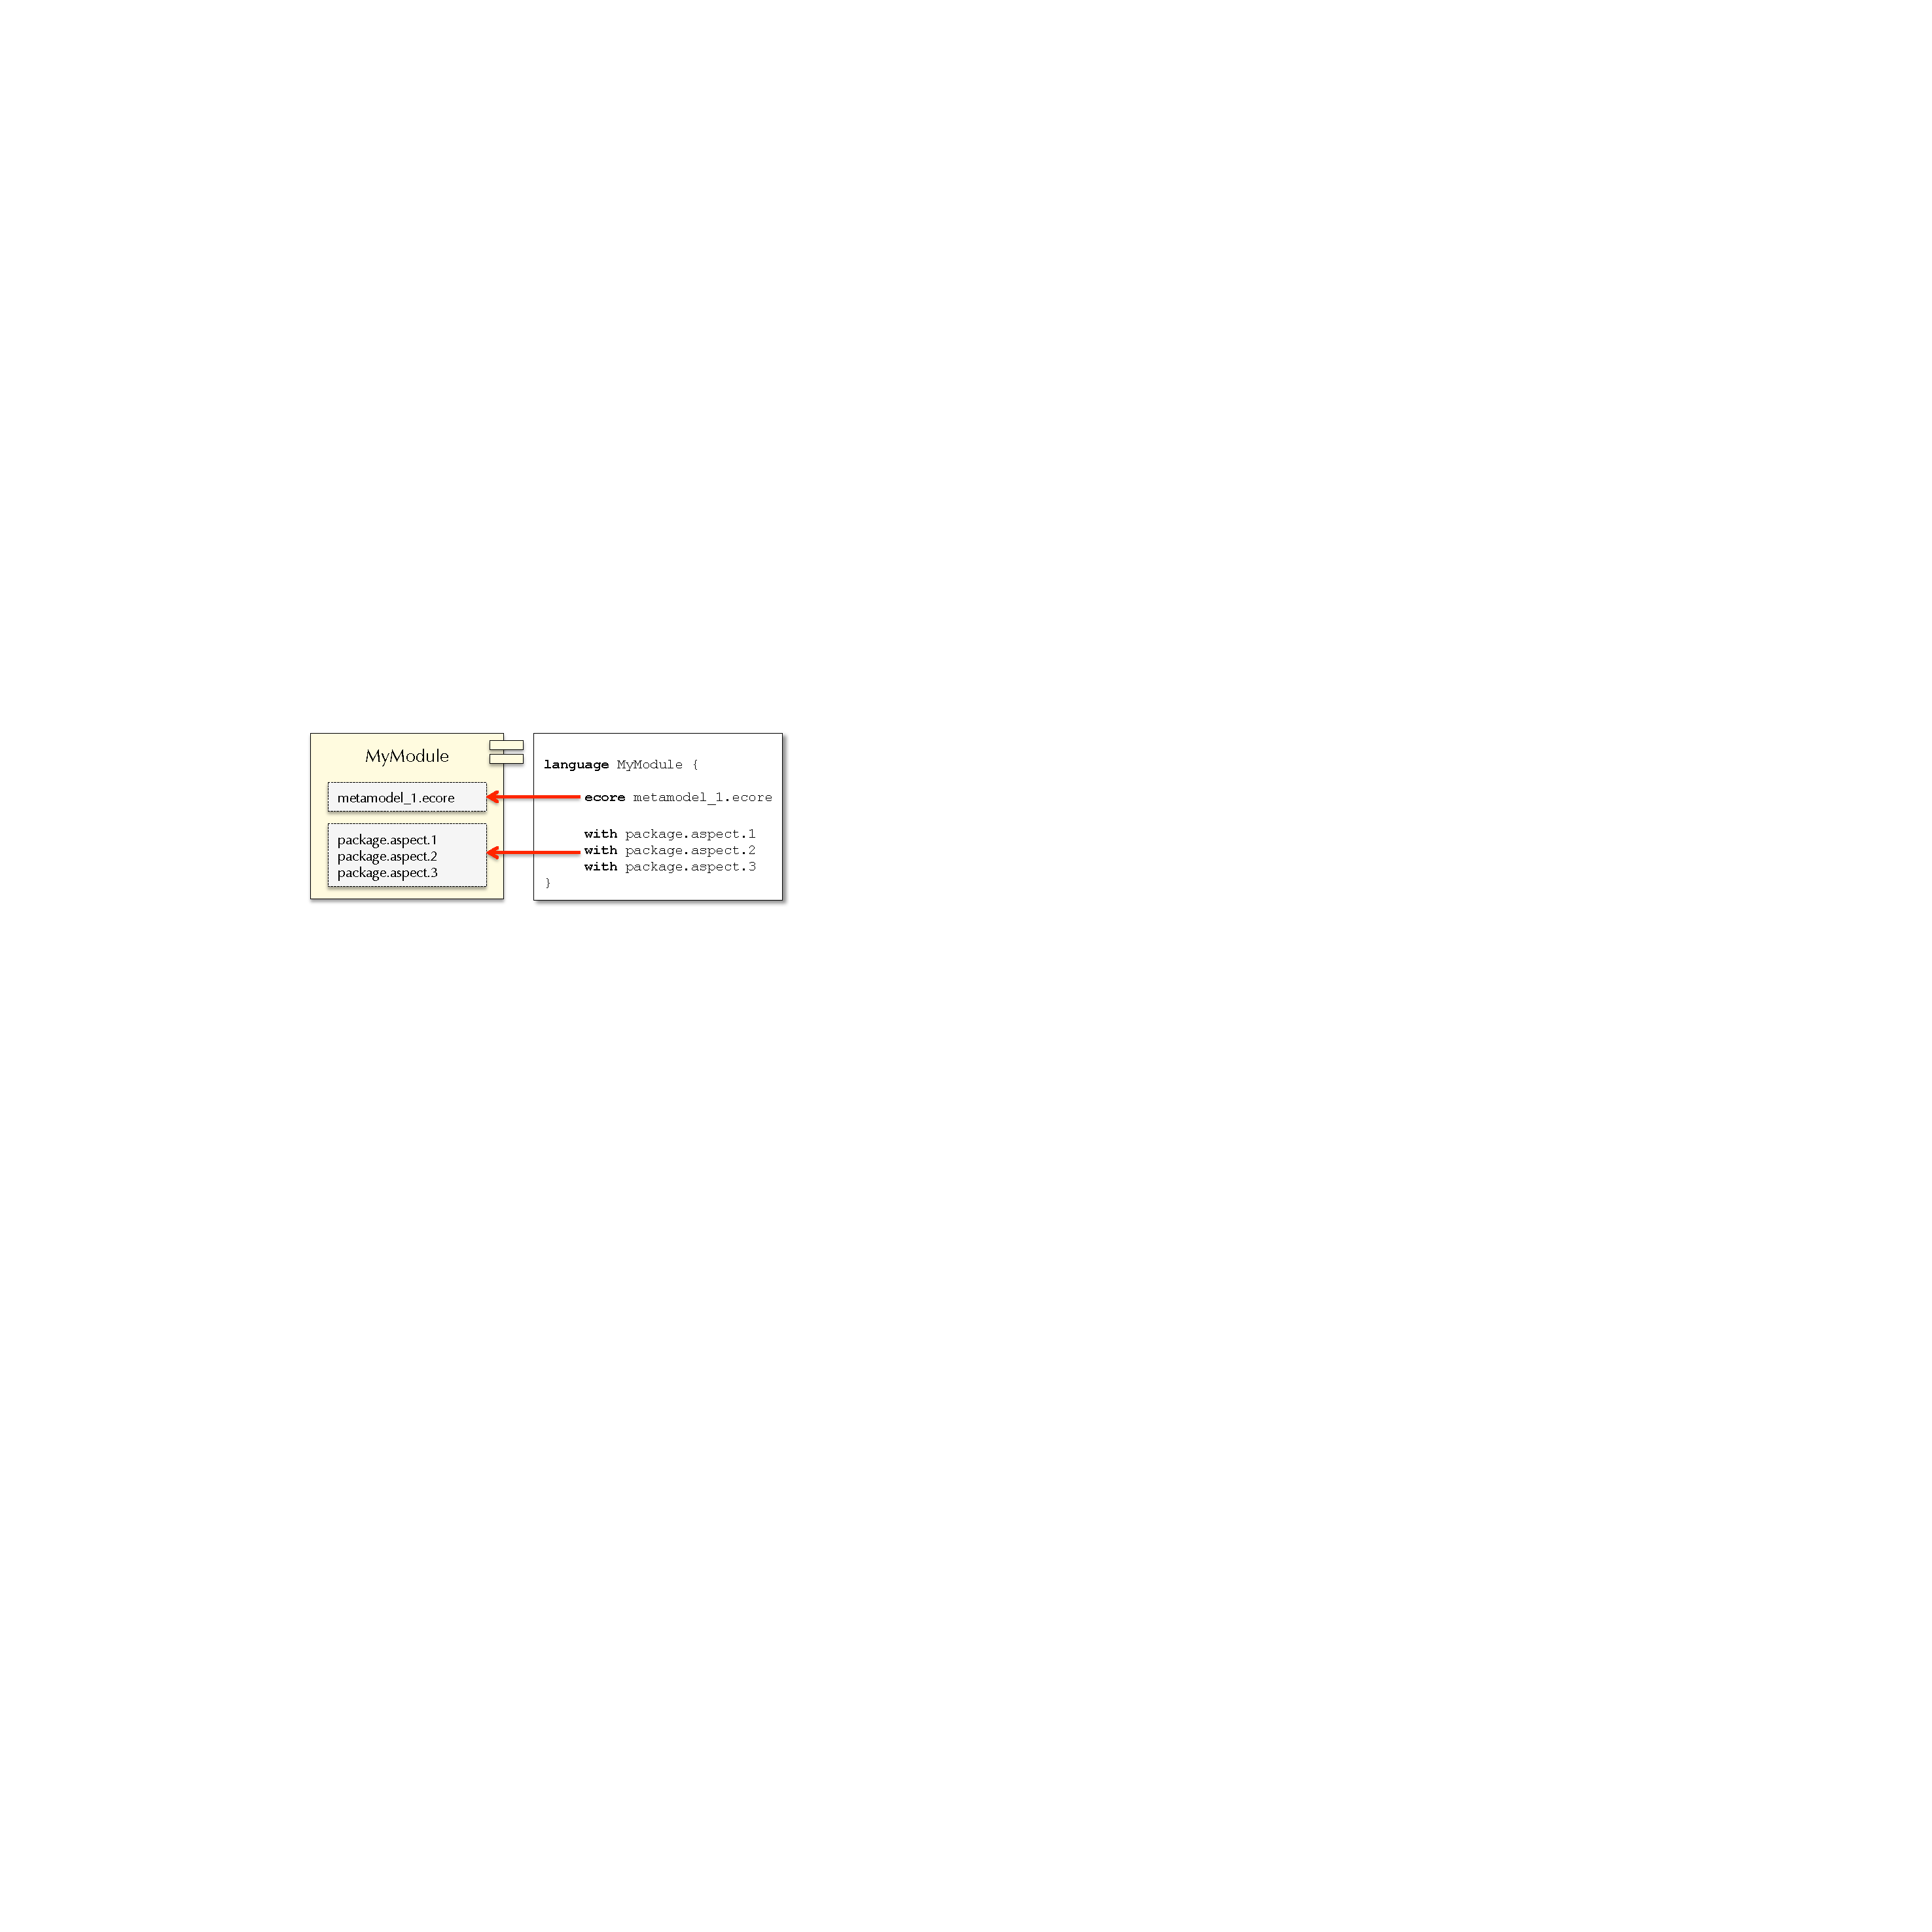
\includegraphics[width=0.8\linewidth]{images/module-melange}
%\caption{Using Melange for weaving metamodels and aspects}
%\label{fig:module-melange}
%\end{figure}

\section{Motivation and problem statement}

\subsection{Illustrating scenario}

Consider a team of language designers that conducts the construction of the DSLs for state machines presented in the last section. During that process, language designers implement the language constructs typically required for expressing finite state machines: states, transitions, events, and so on. In addition, the DSL provides a constraints language that permits to express guards on the transitions. The DSL also provides an expressions language that allows to specify actions on the states of the state machine. 

After being released their DSL for state machines, the language development team is required again. This time the objective is to build a DSL for manipulating the traditional Logo turtle which is often used in elementary schools for teaching the first foundations of programming \cite{Olson:1987}. The new DSL is essentially different from the DSL for state machines. Instead of states and transitions, Logo offers some primitives (such as \texttt{Forward}, \texttt{Backward}, \texttt{Left}, and \texttt{Right}) to move a character (i.e., the turtle) within a bounded canvas. However, Logo also requires an expressions language. In this case, expressions are needed to express more complex movements. For example, by using arithmetic computations.

As illustrated in Figure \ref{fig:cloning}, the typical solution to this type of situations is to replicate the code in a second DSL. Language designers usually copy/paste the segment of the specification that they can reuse. As a result, we have many clones that are expensive to maintain. Naturally, this situation is repeated each time that there is a new DSL to build. Thi fact is illustrated in the Figure \ref{fig:cloning} by introducing a third DSL for expressing flowcharts. In this case, the new DSL requires both, expressions and constraints languages. 

\begin{figure}
\centering
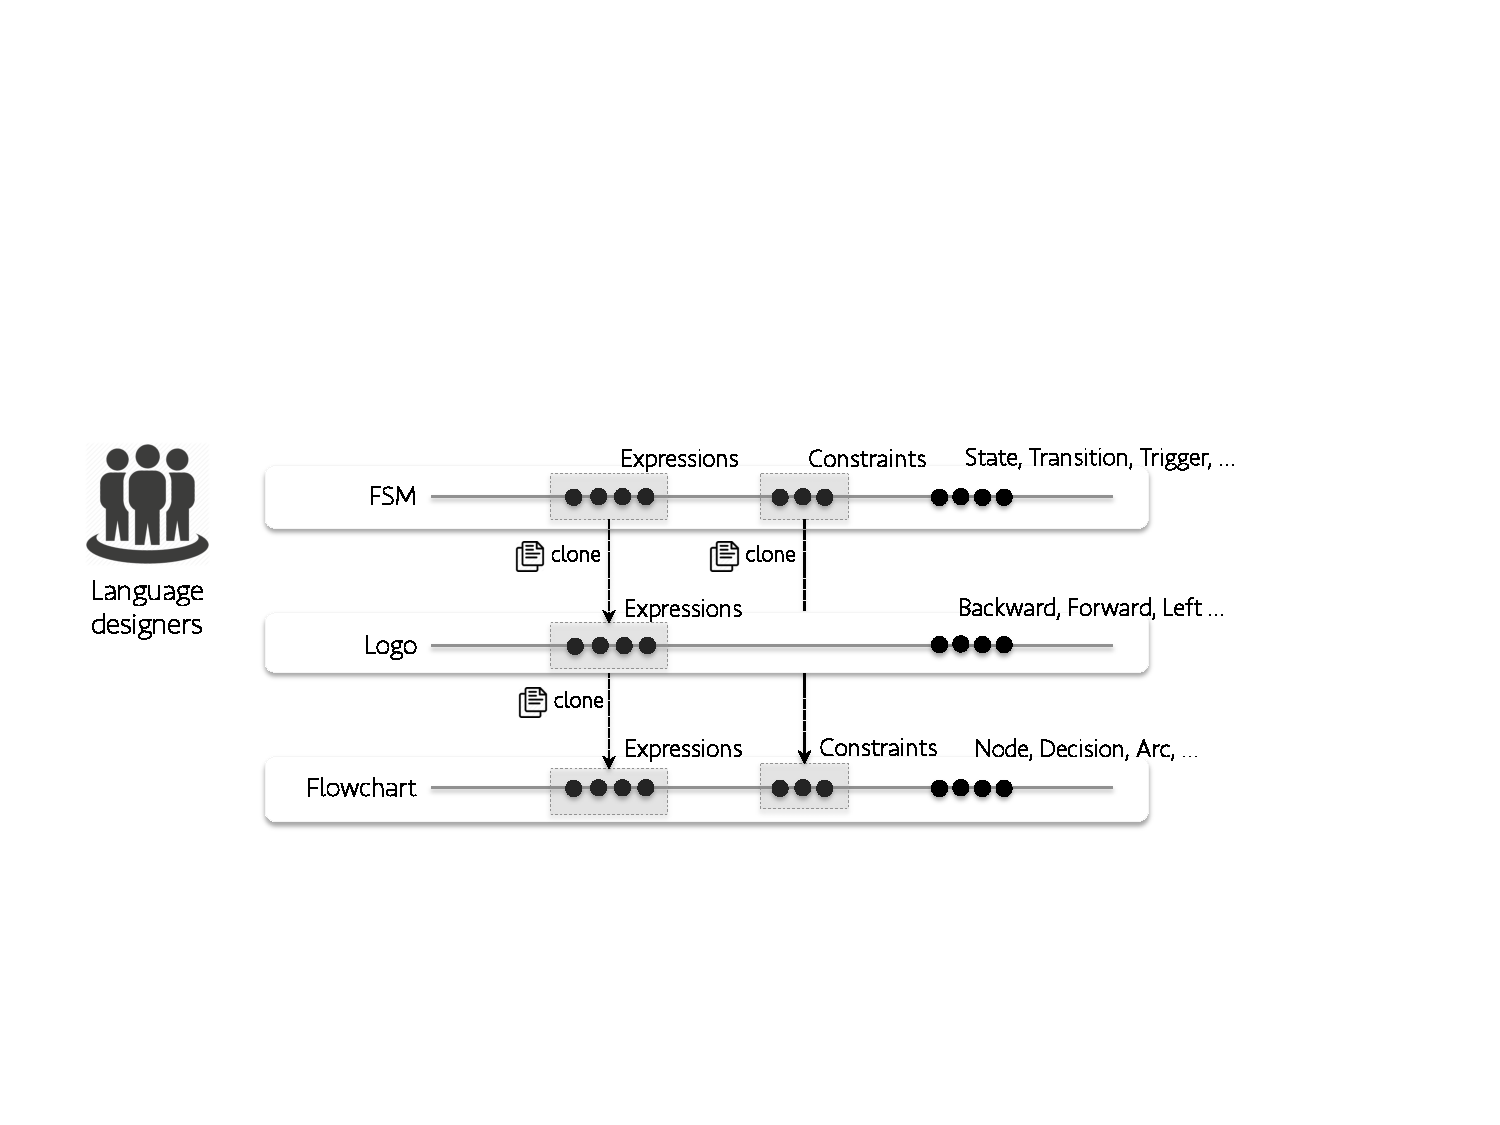
\includegraphics[width=1\linewidth]{images/cloning.pdf}
\caption{Cloning in DSLs development process}
\label{fig:cloning}
\end{figure}

%As a matter of fact, these DSLs are essentially different. Each of them is focus on a particular domain and offers different language constructs. However, there are syntactic and semantic commonalities that are illustrated in Figure \ref{fig:domains}. All the thee DSLs offer some expressions for modifying variables. In the case of FSM these actions are needed the specification of the actions in the states; in the case of Logo expressions are needed to specity the movement and rotation parameters; and in the case of flowchart expressions are needed to specify the body of actions. In addition, both FSM and Flowchart rely on a constraints language. The former for expressing guards in the transitions and the later for expressing guards of the decisions.



\subsection{Overlapping in DSLs and potential reuse}

The aforementioned phenomenon was previously observed by V\"oelter et al \cite[p. 60-61]{voelter:2013}. In fact, that study demonstrates that although many of the existing DSLs are completely different and tackle independent domains; there are related DSLs with overlapping domains. That is, they share certain language constructs i.e., they have \textbf{commonalities} between them. If two DSLs have commonalities and they are specified in the same technological space and using compatible language workbenches, then there is \textbf{potential reuse} since the specification of those shared constructs can be specified once and reused in the two DSLs \cite[p. 60-61]{voelter:2013}. Naturally, commonalities can be found not only at the level of the syntax but also at the level of the semantics. For the technological space discussed in this paper, syntactic commonalities appear where DSLs share some metaclasses and semantic commonalities appear where DSLs share some domain-specific actions.

Figure \ref{fig:domains} illustrates the phenomenon in our illustrating scenario. Note that each DSL is specified in terms of a set of metaclasses (top of the figure), and a set of aspects (bottom of the figure) that weave some domain-specific actions to the metaclasses. In the case of this example, the semantics of the metaclasses expression and constraints are also shared. That means that the semantics are the same. 

It is worth to mention that the fact that two metaclasses are shared does not imply that all their domain specific actions are the same. We refer to that phenomenon as \textbf{semantical variability}. There are two constructs that share the syntax but that differ in their semantics. In such case, there is potential reuse at the level of the syntax since the metaclass can be defined once and reused in the DSLs but the semantics should be defined differently for each DSLs. 

\begin{figure}
\centering
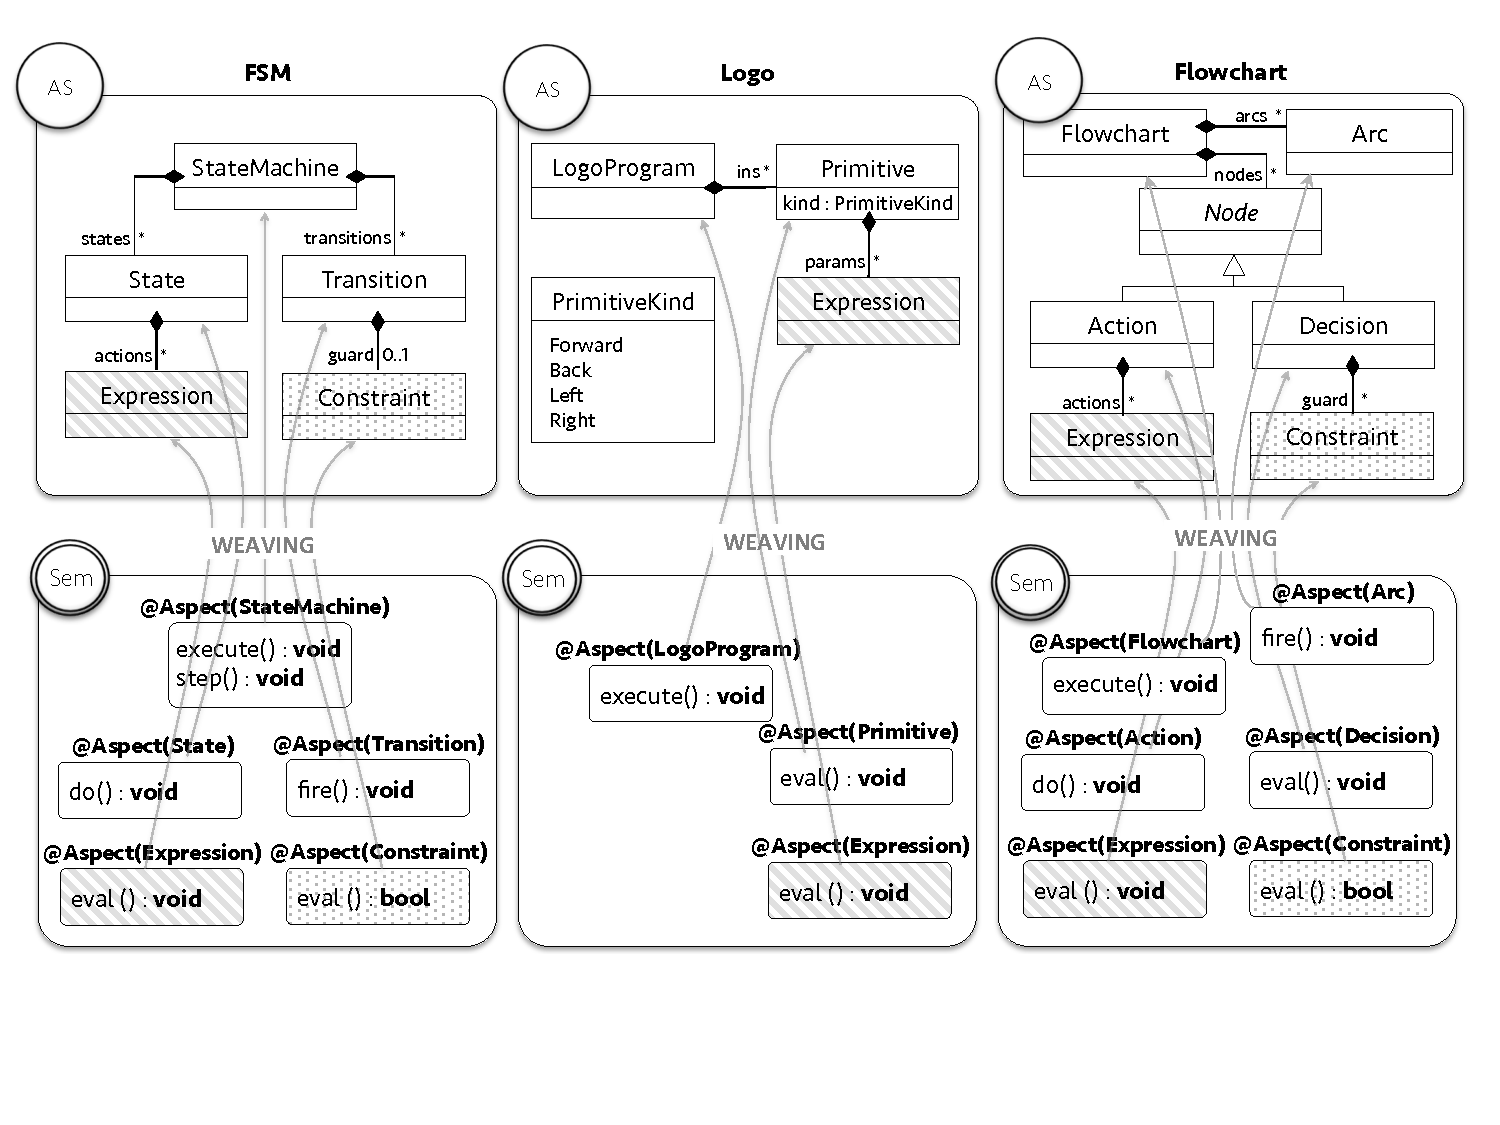
\includegraphics[width=1\linewidth]{images/domains-fig.pdf}
\caption{Commonalities between domains and potential reuse}
\label{fig:domains}
\end{figure}

%Commonalities can be found between two ore more DSLs of the input set. That is, we can find metaclasses and domain specific actions that are shared by more than two DSLs. Hence, intersections should be searched among all the possible combinations of the DSLs in the input set. Once those functions are defined and implemented, the second phase is to use them in order to find the intersections among the DSLs of the input set. 



%there are three DSLs DSLs that are totally independent. That means that they do not share any of their language constructs, and consequently, there is not potential reuse between them. Differently, the two DSLs shown at the right of the figure have overlapping domains. That means that there are a subset of language that are \large\textbf{``equal'' }\normalsize in both DSLs. Note that if two language constructs are the same, we can assume that their specifications are equal and can be reused instead of being replicated.




%Moreover, there are set of DSLs for which the domains can be hierarchically organized \cite[p. 60-61]{voelter:2013}.

%\subsection{Equivalence between language constructs}

%So far, we have based the notion of potential reuse in DSLs on the commonalities existing in a set of DSLs. Nevertheless, this assumption supposes that we are able to compare two language constructs in order to know if they are equivalent. So, now we need to define this \textit{equivalence} relationship. In particular, the comparison of two language constructs relies on two dimensions: (1) comparison of the meta-classes in the abstract syntax; and (2) comparison of the domain-specific actions in the semantics.

